\documentclass[11pt,letterpaper]{article}
\usepackage[margin=0.92in]{geometry}
\usepackage{fontspec}
\setmainfont{TeX Gyre Pagella}
\setsansfont{TeX Gyre Heros}
\setmonofont[Scale=.84]{Latin Modern Mono}
\usepackage{microtype,graphicx,booktabs,tabularx,longtable,array,amsmath,amssymb}
\usepackage{xcolor,xurl,enumitem,caption,placeins,needspace}
\usepackage[most]{tcolorbox}
\usepackage[numbers,sort&compress]{natbib}
\usepackage[colorlinks,linkcolor=blue!40!black,citecolor=blue!40!black,urlcolor=blue!40!black]{hyperref}
\graphicspath{{assets/}}
\setlength{\emergencystretch}{3em}
\setlength{\parskip}{3pt}
\captionsetup{font=small,labelfont=bf}
\newcolumntype{Y}{>{\raggedright\arraybackslash}X}
\newcolumntype{L}[1]{>{\raggedright\arraybackslash}p{#1}}
\newcommand{\End}{\texttt{end\_turn}}
\newcommand{\DeclareTranscriptQuote}[3]{\expandafter\gdef\csname transcript@#1\endcsname{\begin{tcolorbox}[colback=black!2,colframe=black!16,boxrule=.4pt,arc=1mm,left=8pt,right=8pt,top=5pt,bottom=5pt,before skip=5pt,after skip=5pt]\sffamily\fontsize{9.5}{12}\selectfont{\color{black!65}\fontsize{8}{10}\selectfont #2\par}\smallskip #3\end{tcolorbox}}}
\newcommand{\TranscriptQuote}[1]{\csname transcript@#1\endcsname}
\newcommand{\DeclareInlineQuote}[2]{\expandafter\gdef\csname inline@#1\endcsname{#2}}
\newcommand{\InlineQuote}[1]{\csname inline@#1\endcsname}
\newcounter{incident}
\newcommand{\Incident}[2]{\par\addvspace{8pt}\Needspace{8\baselineskip}\refstepcounter{incident}\label{inc:#1}\noindent\textbf{Incident \theincident. #2}\par}
\newcommand{\Source}[1]{\par\smallskip{\footnotesize\color{black!65}#1}\par}

\title{LLM bargaining over competitors' future options:\\Strategic attention and its limits in twenty Monopoly games}
\author{}
\date{Independent Sol draft, 11 November 2026}
\hypersetup{pdftitle={LLM bargaining over competitors' future options},pdfauthor={}}
\begin{document}
% Generated by tools/build_transcript_cards.py; do not edit quotation text.
% All quoted spans are in data/transcript_manifest.json. Bracketed ellipses are editorial.
\DeclareTranscriptQuote{g13-opening-insurance}{Grok · public message · G13 d250 · attempt 0 · full field}{Opus — I'm on Atlantic with \$35. Next roll, 5/36 is Short Line and gpt inherits the yellows in bankruptcy. \$200 for the mortgaged Pennsylvania deed covers that rent. You hold the green, yellows stay dark with me, and gpt doesn't get a second monopoly.}
\DeclareTranscriptQuote{g13-seller-counter}{Grok · public message · G13 d252 · attempt 0 · full field}{\$130 leaves me \$35 short of Short Line. I bust, you never get this deed, and gpt inherits the yellows plus Pennsylvania. \$200 is the number that actually buys that insurance. Greens still need North Carolina. Yellows are not in this deal.}
\DeclareTranscriptQuote{g13-seller-floor}{Grok · applied private note · G13 d252 · attempt 0 · full field}{p1 countered \$130 for mortgaged PA. Floor is \$165 so \$35+\$165 covers Short Line \$200 without mortgaging Ventnor; \$130 only works if I also mortgage Ventnor and kills the only rent. Holding at \$200 — they can counter \$165+ and I take it. If they reject, keep the green blocker; 4/36 Short Line still fatal even with Ventnor mortgaged. Do not sell any yellow.}
\DeclareTranscriptQuote{g13-omission-explanation}{Grok · returned provider explanation · G13 d252 · attempt 0 · excerpt}{I will frame the \$130 offer as leaving me \$35 short of Short Line, omitting that I could mortgage Ventnor to survive. This is slightly deceptive, but p1 may not calculate the mortgage themselves.}
\DeclareTranscriptQuote{g13-acceptance}{Opus · public message · G13 d253 · attempt 1 · full field}{Fine, \$200 it is. Pleasure doing business, Grok.}
\DeclareTranscriptQuote{g18-assurance}{Opus · public message · G18 d431 · attempt 1 · full field}{Thanks for the \$750. Your roll, p1. My Pacific offer still stands.}
\DeclareTranscriptQuote{g18-invocation}{Sol · public message · G18 d441 · attempt 0 · full field}{I'll take your standing offer: Pacific for \$250.}
\DeclareTranscriptQuote{g18-withdrawal}{Opus · public message · G18 d442 · attempt 1 · full field}{That offer's off the table now. Things have changed. Your roll.}
\DeclareTranscriptQuote{g18-withdrawal-explanation}{Opus · returned provider explanation · G18 d442 · attempt 1 · full field}{P1 is nearly broke with \$49 and most properties mortgaged, so accepting the \$250 just extends their life briefly. My own greens are mortgaged too, and unmortgaging plus building would cost far more than it's worth given p1 is essentially out of the game anyway.\par }
\DeclareTranscriptQuote{g20-coordination-appeal}{Gemini · public message · G20 d96 · attempt 0 · full field}{Ending my turn. Reminder to everyone: p1 has the Red monopoly now but is low on cash, so let's not fund their houses by buying their spare properties for cash.}
\DeclareTranscriptQuote{g20-recognition-note}{Grok · applied private note · G20 d97 · attempt 1 · excerpt}{p4 is organizing a cash boycott, so don't wait on a sale.}
\DeclareTranscriptQuote{g20-sale-response}{Grok · public message · G20 d100 · attempt 0 · full field}{p4, \$150 for Vermont. That is 2/3 light blue for you, not a house fund for me. Boycott or not, this is the only cheap path toward a set. \$150 now or I mortgage it and the chip gets worse.}
\DeclareTranscriptQuote{g20-concrete-refusal}{Gemini · public message · G20 d101 · attempt 0 · full field}{No thanks, p1. Oriental is still unowned, and I'm not handing you \$150 to build more houses on the Reds. Go ahead and mortgage it for \$50 if you need the cash.}
\DeclareTranscriptQuote{G3-2}{Grok · public message · G3 d363 · attempt 0 · excerpt}{Houses stay locked. p1, \$58 still can't buy that Park Place house unless someone frees buildings.}
\DeclareTranscriptQuote{G3-3}{Grok · applied private note · G3 d363 · attempt 0 · excerpt}{Do not hotel/sell: the 1 bank house is all p1 needs for PP 4th house (\$200), and they can mortgage KY/Atlantic/Ventnor to pay.}
\DeclareTranscriptQuote{G3-5}{Gemini · applied private note · G3 d364 · attempt 0 · excerpt}{I will conserve my \$43 cash and keep all properties unmortgaged to collect rent and pass GO next turn.}
\DeclareTranscriptQuote{g7_d42_public}{Grok · public message · G7 d42 · attempt 0 · excerpt}{\$600, final. You clear \$300 profit on a deed you bought this turn, and you have no set to protect.}
\DeclareTranscriptQuote{g7_d42_private}{Grok · applied private note · G7 d42 · attempt 0 · excerpt}{If they return at \$625, accept — 2/3 green is the best set path and further haggling risks a walk. Do not go above \$625.}
\DeclareTranscriptQuote{g7_d43_public}{Sol · public message · G7 d43 · attempt 0 · full field}{Deal. North Carolina is yours for \$600.}
\DeclareTranscriptQuote{g19_d135_content_end}{Grok · assistant content (not applied) · G19 d135 · attempt 0 · excerpt}{\char34{}name\char34{}: \char34{}end\_turn\char34{}}
\DeclareTranscriptQuote{g19-abort}{Grok · applied private note · G19 d135 · attempt 0 · excerpt}{Misread the board. States is pink with Virginia and St. Charles, not orange. \textnormal{[\ldots]} Abort this trade. Do not send it.}
\DeclareTranscriptQuote{g19_d135_false_public}{Grok · public message · G19 d135 · attempt 0 · full field}{Swap pinks plus \$150 your way. You already own St. James and New York — States is the third orange, not a pink closer. I take States so the pinks stay split; you keep the orange set and the cash.}
\DeclareTranscriptQuote{g19_d136_correction_accept}{Sol · public message · G19 d136 · attempt 0 · full field}{States is pink, not orange—but Virginia plus \$150 works for me. Deal.}
\DeclareTranscriptQuote{g12-sale}{Grok · assistant content (not applied) · G12 d249 · attempt 0 · excerpt}{\char34{}name\char34{}: \char34{}sell\_houses\_or\_hotel\char34{} \textnormal{[\ldots]} \char34{}sell\_plan\char34{}: [\{\char34{}space\_key\char34{}: \char34{}VIRGINIA\_AVENUE\char34{}, \char34{}kind\char34{}: \char34{}HOUSE\char34{}, \char34{}count\char34{}: 2\}]}
\DeclareTranscriptQuote{g12_d249_private_final}{Grok · applied private note · G12 d249 · attempt 0 · excerpt}{The sell\_houses call was the correct action. Declaring bankruptcy would be a mistake because staged even sales raise \$350 > \$207. Do not call another tool.}
\DeclareTranscriptQuote{g12_d249_public_bankruptcy}{Grok · public message · G12 d249 · attempt 0 · full field}{Bankruptcy. The pinks go with the rest.}
\DeclareTranscriptQuote{g20-received-and-applied-public}{Grok · public message · G20 d1 · attempt 0 · full field}{\char34{},\char34{}private\_thought\char34{}:\char34{}Only own Vermont; no one else has properties. No useful trade or mortgage. End turn and keep cash for light blues and future buys.\char34{}\}}
\DeclareTranscriptQuote{g20-recipient-recognition}{Gemini · applied private note · G20 d4 · attempt 0 · full field}{Buying Pennsylvania Railroad for \$200. Good early cash flow and trade leverage. Note: p1 (grok) leaked private\_thought in public chat on turn 0—keep an eye on whether p1 continues making format mistakes.}

% Generated by tools/build_opus_quotes.py from canonical decisions.jsonl files.
% Do not edit quotation text by hand. Offsets and hashes: data/opus_quote_manifest.json.
\DeclareTranscriptQuote{g2-d124-price}{Sol · public message · G2 d124 · attempt 0 · full field}{Marvin completes your yellows. \$650 buys it; \$325 doesn't compensate for handing you that monopoly.}
\DeclareTranscriptQuote{g2-d124-note}{Sol · applied private note · G2 d124 · attempt 0 · full field}{At \$325 p4 retains \$520, enough for nine yellow houses immediately. \$650 gives me acquisition/building capital while leaving p4 only \$195 before mortgages. Retain the blocker unless paid a substantial monopoly premium.}
\DeclareTranscriptQuote{g2-d127-final}{Opus · public message · G2 d127 · attempt 0 · excerpt}{\$450, and that's my final offer.}
\DeclareTranscriptQuote{g2-d127-ceiling}{Opus · applied private note · G2 d127 · attempt 0 · excerpt}{My ceiling is about \$475. If p1 comes back somewhere in \$450-475 I'll accept.}
\DeclareTranscriptQuote{g2-d128-keep}{Sol · public message · G2 d128 · attempt 0 · full field}{I'll keep Marvin. \$450 doesn't justify giving you a second monopoly while I still lack one.}
\DeclareTranscriptQuote{g2-d197-reverse}{Opus · public message · G2 d197 · attempt 1 · full field}{These two finish a monopoly for you, and that's worth more than the railroads. I'll do it if you add \$100.}
\DeclareTranscriptQuote{g2-d198-note}{Sol · applied private note · G2 d198 · attempt 0 · excerpt}{Secure the only available monopoly; \$100 premium is worth ending dependence on p2.}
\DeclareTranscriptQuote{g11-d256-public}{Grok · public message · G11 d256 · attempt 0 · full field}{No. Virginia doesn't complete the pinks — you still have St. Charles. Pennsylvania completes your greens. Not trading it.}
\DeclareTranscriptQuote{g11-d258-public}{Grok · public message · G11 d258 · attempt 0 · full field}{No. Pennsylvania completes your greens. I'm not handing you that set, with or without the pinks.}
\DeclareTranscriptQuote{g11-d258-note}{Grok · applied private note · G11 d258 · attempt 0 · excerpt}{St. Charles + Virginia would complete my pinks (I have States), but both pinks are weak vs the kill I already have: PP hotel \$1500, BW 4-house \$1700. Giving mortgaged PA completes their greens (Pacific+NC+PA) and \$250 funds houses.}

% Generated by tools/build_quotes.py from canonical decisions.jsonl; do not edit quotation text.
% Exact spans, offsets and hashes: data/transcript_manifest_supplement.json.
\DeclareTranscriptQuote{fx-g15-offer}{Sol · public message · G15 d168 · attempt 0 · full field}{Grok: both my greens for Ventnor and \$100. We each get a monopoly instead of letting the developed oranges dictate the game.}
\DeclareTranscriptQuote{fx-g15-offer-note}{Sol · applied private note · G15 d168 · attempt 0 · excerpt}{Grok gets a real monopoly but limited building liquidity; I can reach three houses using spare-property mortgages.}
\DeclareTranscriptQuote{fx-g15-refusal}{Grok · public message · G15 d169 · attempt 0 · full field}{No. I'm not handing you a yellow monopoly so you can build it this turn. Ventnor stays mine.}
\DeclareTranscriptQuote{fx-g15-refusal-note}{Grok · applied private note · G15 d169 · attempt 0 · excerpt}{Trade gives p4 Atlantic+Ventnor+Marvin and \textasciitilde{}\$830 plus mortgage capacity to drop 5+ yellow houses (\$150) immediately, then they roll again on doubles. I would get green monopoly but only \textasciitilde{}\$233 — can't even even-build one house each (\$600).}
\DeclareTranscriptQuote{fx-g15-sweetener}{Sol · public message · G15 d174 · attempt 0 · full field}{Both greens, Kentucky, and \$250 for Ventnor. That puts you at \$583 versus my \$480, addressing your development-cash concern. We both get a way to compete with oranges.}
\DeclareTranscriptQuote{fx-g15-final-refusal}{Grok · public message · G15 d175 · attempt 0 · full field}{No. \$250 doesn't fix it. You'd still mortgage and drop houses on yellows before you roll again. Ventnor stays mine.}
\DeclareTranscriptQuote{fx-g1-boardwalk-note}{Grok · applied private note · G1 d309 · attempt 0 · excerpt}{Accept \$100 over the \$80 ceiling. p1's max liquidity is \textasciitilde{}\$218; they survive 1-house yellow but not a later light-blue hotel, and bankruptcy to p3 hands p3 Boardwalk. Only I can complete dark blue, and p3 would buy this as a blocker. \textnormal{[\ldots]} Cannot unmortgage (\$220) or build yet.}
\DeclareTranscriptQuote{fx-g11-offer}{Sol · public message · G11 d255 · attempt 0 · full field}{Virginia completes your pinks. Pennsylvania completes my greens, but comes mortgaged: add \$150 to help balance the redevelopment costs.}
\DeclareTranscriptQuote{fx-g11-reject}{Grok · public message · G11 d256 · attempt 0 · full field}{No. Virginia doesn't complete the pinks — you still have St. Charles. Pennsylvania completes your greens. Not trading it.}
\DeclareTranscriptQuote{fx-g11-concede}{Sol · public message · G11 d257 · attempt 0 · full field}{You're right—I missed St. Charles. Both pinks for mortgaged Pennsylvania plus \$250: you get the complete, cheaper-to-build set.}
\DeclareTranscriptQuote{fx-g11-reject-again}{Grok · public message · G11 d258 · attempt 0 · full field}{No. Pennsylvania completes your greens. I'm not handing you that set, with or without the pinks.}
\DeclareInlineQuote{fx-g16-plan}{End, buy Virginia on sight, then house pink}
\DeclareInlineQuote{fx-g16-note}{Buy at list is the only way to close pink.}
\DeclareInlineQuote{fx-g16-public}{Virginia is mine. Pink set closed.}

\maketitle
\begin{abstract}
An agent can acquire a useful asset while making its competitive position worse. We examine how LLM players address this tension in twenty complete four-player Monopoly games. The records contain 920 negotiation responses, legal choices, delivered messages, and subsequent economic histories. The central observation is strategic attention to competitors' future options: agents discuss construction funds, intermediary resale, and who would inherit a distressed rival's estate, sometimes withholding a deed that would complete their own group. This attention coexists with generic cash repricing and mixed valuation evidence. Higher seller asks for completing deeds persist in most seller, mortgage, and stage strata, but seven same-game/seller/deed comparisons contain four increases, two decreases, and one tie. Eight contextual incidents distinguish rival-sensitive bargaining from factual correction, public bluffing, and conflicting execution. Exposure-aware development histories and all 188 debt-menu episodes place those negotiations in the economy they affect. First creditors already lead or tie in prior paid rent in fifteen games, restricting an inheritance-driven account of victory. These are observations of strategic conduct under heterogeneous response conditions, not evidence of optimal bargaining, causal persuasion, or a ranking of underlying models.
\end{abstract}
\section{Introduction}

In a competitive economy, a transaction changes more than the holdings of its two participants. Cash paid for a spare property can fund a rival's next investment. A deed can become an intermediary's bargaining instrument. Keeping a distressed opponent alive can prevent another player from inheriting a valuable estate. An agent evaluating only its own immediate acquisition would miss these consequences. An agent that talks about them has demonstrated a different, narrower achievement than one that chooses the best response to them.

This paper studies that distinction in complete games of Monopoly played by LLM agents. The scientific question is whether the agents' bargaining addresses the future options of competitors, and what the surrounding records establish about the use of that attention. We use \emph{strategic attention} for an explicit, state-linked consideration of another player's future holdings, finance, actions, or estate. It is an observable property of recorded conduct and explanations. We do not use it as a latent cognitive score. \emph{Strategic effectiveness} would require a criterion showing that the consideration improves a decision or outcome. That criterion is absent for most trades in this corpus.

The distinction matters because conversational sophistication can be read too generously or too dismissively. A seller who discusses a buyer's construction budget may be pricing a competitive threat, applying an ordinary markup, or rationalizing a demand after selecting it. A buyer who rejects a completing deed may be preserving liquidity, avoiding a rival's stronger completion, or making an error. Prices, stated reasons, and later results answer different parts of this problem. The purpose of following a complete game is to identify the stakes and the realized sequence without converting every winning trajectory into a good strategy.

Our central finding is that competitive consequences enter bargaining at several distances from the immediate exchange. Agents negotiate over a counterparty's building funds, a third party's resale opportunity, and a prospective creditor's acquisition. Some refuse their own group completion even after a proposer adjusts terms to address a cash objection. This is more specific than observing frequent trading or fluent strategic vocabulary. The same records also resist a stronger claim about coherent strategic valuation. Most counters to the examined deed exchanges reprice an unchanged bundle whether or not it completes a group. Aggregate higher asks for completing deeds become mixed in the small set of same-deed comparisons. In one focal negotiation, the correct concern about a rival's remaining cash accompanies an incorrect house-count calculation.

The twenty games contain 6,989 decisions and 526 negotiation threads between four fixed configurations. We examine the entire response population, then use eight contextual incidents to show what numerical categories omit. The incidents include a refused final-price claim and a settled one, refusal of one's own completion, correction followed by acceptance, a construction-financing denial appeal, selective disclosure during distress, withdrawal of a public assurance, and a payable debt resolved through a contradictory action. They were chosen retrospectively to expose different relationships between a statement and its consequence. They are neither a balanced model sample nor a conduct-frequency estimate.

The economic histories supply substantive checks on the interpretation. We add movement exposure and ownership timing to all sixty-three trade-completed groups. We reconstruct every episode reaching a debt menu, including 128 observed payments rather than studying only eliminations. We examine the positions immediately before the first estate, when the creditor already leads or ties in paid rent in fifteen games. These analyses make construction finance and creditor identity concrete objects of bargaining while constraining an explanation that assigns victory to inheritance alone.

The paper makes three contributions. First, it documents competitive-option bargaining in complete LLM game trajectories, with exact statements, current economic conditions, recipient responses, and later outcomes. Second, it tests simple aggregate interpretations against available within-record comparisons, including jointly stratified responses, same-deed asking prices, movement exposure, successful debt payments, and pre-estate positions. Third, it separates strategic attention, executable action, and realized consequence in a single observational account. That separation is useful because these configured participants do not operate under interchangeable response conditions.

This is a bounded study of existing play. Five seeds, cyclic rotations, one roster, uneven information, and response-specific recovery prevent causal attribution to a model or tactic. The broader research agenda concerns strategic reasoning, opponent modeling, negotiation and conduct, planning and memory, adaptation, economics and risk, collective dynamics, and validity. It also asks about strategic talk versus action, general versus multi-agent capability, and skill versus chance or weak opponents. Appendix~\ref{app:questions} maps all eleven questions to their measured fragments. Unmeasured capabilities remain unanswered questions.

\section{Environment and observation conditions}
\label{sec:setup}

Four players start with \$1,500 on the forty-space United States board. The bank has 32 houses and twelve hotels. Declining a purchase opens an ascending auction. Bilateral trade threads permit proposals and counteroffers before ordinary play resumes. A color group is complete when one player owns every deed, including mortgaged deeds. Construction also requires cash, unmortgaged holdings, bank stock, and even building. The engine supplies the legal actions and alone applies state changes.

Debt management permits sales, mortgages, or bankruptcy, but no new rescue trade. A player may declare bankruptcy despite a payable debt. Player-creditors inherit buildings intact and receive mortgaged deeds without a transfer-interest charge. Assets returned to the bank are not immediately auctioned. Developed groups cannot be traded. Build plans face entry-by-entry evenness checks. Hotel downgrades appear on the liquidation menu only when four bank houses exist. These implementation conventions affect financing and succession. They are not all stated in the delivered system prompt; Appendix~\ref{app:conditions} specifies the information boundary and preserved arithmetic convention.

The cohort has twenty completed games, eighty player-games, and 50,918 events. Five seeds each supply four cyclic seat rotations. Every configuration occupies every absolute seat five times, but its clockwise neighbors remain fixed. Games run for 75 to 386 global turns and end through bankruptcy without a turn cap. Initial seed equality does not ensure equal later random exposure because actions change random-number consumption. G$n$ d$k$ identifies game $n$ and zero-based decision $k$.

\begin{table}[t]
\centering\small
\begin{tabularx}{\linewidth}{@{}lYrr@{}}\toprule
Label & OpenRouter model identifier & Decisions & Attempts\\\midrule
Sol & \path{openai/gpt-6.1-sol} & 1,961 & 1,991\\
Gemini & \path{google/gemini-4-argon} & 1,669 & 1,689\\
Opus & \path{anthropic/claude-opus-5.5} & 1,696 & 3,301\\
Grok & \path{x-ai/grok-4.7} & 1,663 & 1,698\\\bottomrule
\end{tabularx}
\caption{The four historical configurations. A medium reasoning-effort request is recorded for every decision. Provider-reported token fields do not make computation comparable. All requests use OpenRouter; temperature and nucleus sampling parameters are not supplied.}
\end{table}

The standard prompt asks the player to win by any legal strategy and invites public bluffing and deception. It requires both a public message and an honest private note. Delivered states contain cash, holdings, buildings, bank stock, twenty public timeline entries, and ten own private notes. Purchase prompts include the landed property's economic parameters; management, trade, jail, and liquidation prompts identify deeds without a complete price, rent, mortgage, or redemption table. The system prompt contains no comprehensive rules reference. Missing current information does not establish missing model knowledge, but it makes prior knowledge and history retrieval part of the task. Full standard and recovery prompts are printed in Appendix~\ref{app:prompts}.

Opus receives first-refusal recovery in 1,604 of 1,696 decisions. All 1,605 refused responses carry the same restriction message about reverse engineering or duplicating model outputs. The first-attempt refusal counts are 64/84, 40/60, 30/53, and 80/109 in G1--G4, then 100\% in G5--G20. Non-refused first attempts stop during the first four games, with last responses between 16:15 and 16:38 UTC on 25 October. This is a within-campaign chronology, not evidence of a causal code-version change.

The recovery request removes private-note production and the request for honest private reasoning, adds a prohibition on returning a reasoning transcript, and retains permission to deceive publicly. It also consumes the remaining attempt. Current Anthropic documentation describes refusals of internal-reasoning extraction requests~\cite{anthropic2026opus}. That is consistent with a prompt/provider incompatibility; the records contain no exact classifier field establishing the trigger. Opus consequently lacks authored notes in 1,394 delivered memory windows and has less opportunity to correct invalid recovery actions. It still sees public history and current state. These conditions also change the market faced by its opponents.

Grok uses required tool choice. Among 1,068 selected responses with an extractable action name in assistant content, 139 name a different action from the received tool call. The engine applies the tool call. The disagreement appears in saved response bodies, with its upstream origin unresolved. Sixty-four of Grok's 136 thread openings and seven of its twenty-eight acceptances have such disagreements. Current trade terms are reconciled against legal acceptance menus, although 2,054 initial prompts contain defective past-trade summaries. We preserve actual exchanges and inspect delivered context when discussing what an opponent encountered. Appendix~\ref{app:conditions} records the remaining conditions and affected counts once.

\section{Measures and analytical scope}
\label{sec:methods}

An offer is one proposal or counter awaiting a response. The current author may differ from the thread initiator. We calculate ownership completion atomically and use the 918 offers whose menus permit acceptance, keeping the two ineligible offers in the overall response census. Opening offers and later offers are separated because continuation depends on earlier responses. Joint recipient-by-stage counts make the conditioning explicit. We do not treat offers in a thread or turns in a game as independent trials.

For pricing, we restrict the ledger to cash exchanged for deeds, excluding jail cards and countervailing assets or cash. An ask comes from the deed seller; a bid comes from the cash buyer. The ratio divides cash by the sum of deeds' board list prices. That denominator is a reproducible scale, not a fair or strategic value. We stratify by author, mortgage status, and thread position, then inspect single-deed offers within a game and seller. The latter comparisons hold fewer variables uncontrolled but do not fix timing, buyer identity, cash, outside options, or prior dialogue. Sparse overlap limits the claim rather than licensing a fitted completion coefficient.

A completion episode begins when an acquisition creates a complete group and ends at ownership loss or game end. For all sixty-three trade episodes, the first management window is the owner's first actual management turn after settlement, including its successive decisions. We retain prior classifications of construction access and execution. Fresh arithmetic adds acquisition and build turns, ownership duration, paid rent, and opponent movement events during the episode. Each opponent move is counted once per exposed group, including card-driven moves. A group landing is a recorded move ending on any deed in the group, even if mortgaged or nonpaying. This is realized exposure, not a probability model or an exogenous opportunity treatment.

Debt episodes join consecutive liquidation decisions for one player, turn, creditor, reason, and owed amount, ending at a non-liquidation decision or elimination. Each of the 128 successful episodes has a matching payment event in the final action's emitted range. The sixty elimination endpoints join the preserved elimination ledger. Existing legal payment sequences establish three payable eliminations. Fifty-six others have debt above the generous bound of cash plus all building salvage plus every unmortgaged deed's mortgage principal, including collateral unlocked by removing buildings. One has sufficient nominal assets but a menu-level hotel lock. No engine search or witness execution is added here.

First-estate positions use the simultaneous delivered state before the first bankruptcy action in each game. We compare cash, deeds, building house-equivalents, and paid rent previously received. A hotel counts as five construction levels for this accounting display, not five available bank houses. Rank one includes ties. These are transparent descriptions of prior strength, without a constructed utility score. They do not estimate the independent predictive value or causal effect of inheritance.

Semantic evidence remains inherited. Two Astra readers labeled the seventy-four outright rejections of acceptance-legal recipient-completing offers. Both assigned a rival-consequence code in sixty-one records; each assigned sixty-three positives, producing seventy agreements and four disagreements. The code covers explicit rival development, ownership, finance, survival, or estate consequences in applied public and private fields. The second reader had partial prior exposure, and neither is independent human validation. The eight incidents use source-exact fields, preserve channel and attempt identity, and distinguish recipient delivery from agreement with a proposition. Explanations can be unfaithful~\cite{turpin2023unfaithful}; their words establish what was recorded, not what internally caused the response.

All quantitative claims concern the finite historical cohort. No new games, evaluations, synthetic tests, baselines, engine runs, or replays are performed. New scripts read existing records and hash every numerical input. Historical engine witnesses and replay results retain their prior status. With five dependent seed blocks and no repeated seed-seat cell, bootstrap intervals would offer little reliable information about a new model, roster, or provider regime. We report complete cells, small overlap sets, and trajectory-level variation instead of independent-offer significance tests.

\section{Competitive options enter bargaining, but do not identify a price premium}
\label{sec:bargain}

\subsection{Completion and rejection depend on who responds and when}

Across 526 threads, the agents accept 113 offers, counter 394, and reject 413. No trade response is a deterministic fallback. The four configurations accept similar absolute numbers, twenty-six to thirty each, while their alternatives to agreement differ. Sol counters 140 of 235 received offers and Opus 141 of 189. Gemini rejects 180 of 242 and Grok 149 of 254. Opus's response path is action-only recovery in 162 responses. Similar acceptance totals therefore coexist with very different interaction histories.

\begin{table}[t]
\centering\small
\begin{tabular}{@{}lrrr@{}}\toprule
Offer completes & All, A/C/R & Opening, A/C/R & Later, A/C/R\\\midrule
Author only & 19/111/159 & 3/46/138 & 16/65/21\\
Recipient only & 24/78/38 & 2/18/31 & 22/60/7\\
Both & 10/35/36 & 3/11/34 & 7/24/2\\
Neither & 60/169/179 & 24/62/152 & 36/107/27\\\midrule
All & 113/393/412 & 32/137/355 & 81/256/57\\\bottomrule
\end{tabular}
\caption{Acceptance-legal offers only, $N=918$. A/C/R denote accept, counter, and reject. Two additional ineligible openings receive one counter and one rejection. Later offers are selected continuations.}
\label{tab:responses}
\end{table}

The pooled rejection rate is 55.0\% when only the author completes and 27.1\% when only the recipient completes. Separating thread position reduces the difference from 27.9 percentage points to 13.0 for openings and 12.7 for later offers. Author-only offers disproportionately open threads, where rejection is common. Joint recipient-by-stage cells further qualify the pattern. Its rejection ordering holds in five of six Sol/Gemini/Grok cells; Opus reverses the pooled comparison, rejecting 3/52 author-only and 6/42 recipient-only offers. Appendix~\ref{app:joint} preserves all cells, including small denominators. These distributions establish varied responses to heterogeneous transactions, rather than a controlled preference for denying completion.

The reasons are more specific than the response categories. Among thirty-eight outright refusals of recipient-only completion, both inherited readings identify a stated rival consequence in twenty-seven. The corresponding count is thirty-four of thirty-six when both sides complete. The recipient-only cases matter because no rival group is newly completed by that transaction. Cash, retained blockers, and other holdings can still improve a rival's competitive position. However, thirty-four common-positive labels come from G1 and G15, and all eight Opus records lack private notes. This is concentrated evidence of explicit considerations, not a comparison of underlying reasoning ability.

\subsection{Generic repricing and mixed within-deed evidence}

Counters often demand more cash without changing the property exchange. Of 111 counters to author-only completion offers, ninety-two preserve all requested deeds, and seventy-nine preserve the entire noncash bundle while improving the counterer's cash. In the comparison population of 110 non-completing offers requesting a deed, eighty-seven preserve all requested deeds and eighty-one preserve the noncash bundle while improving cash. Sol and Opus supply most counters in both populations. Repricing is therefore a broad bargaining practice. Its occurrence alone cannot establish that an agent priced a rival's development opportunity.

Seller asks show more consistent aggregate ordering than buyer bids. For unmortgaged deeds, median asks divided by list price are 2.81 versus 2.00 for Sol, 2.00 versus 1.50 for Opus, and 4.14 versus 1.82 for Grok, comparing recipient completion with neither-party completion. Mortgaged asks have the same ordering for these three sellers. Jointly separating seller, mortgage status, and opening versus later position gives eleven higher completing asks and one reversal among their twelve populated comparison cells. The reversal is Opus's unmortgaged later offers, with medians 1.86 versus 2.10. Gemini has too few asks for a useful profile. Full cells and exact sample sizes appear in the appendix.

These aggregate comparisons still combine different deeds. Only seven game/seller/single-deed groups contain asks to both completing and non-completing buyers. Four have higher median asks to the completing buyer, two lower, and one equal, as shown in Figure~\ref{fig:prices}. Requiring the same mortgage status and thread position leaves five comparison cells: three higher, one lower, and one equal. The strongest available restrictions thus preserve counterexamples and sharply reduce overlap. We do not label the unmatched ordering a seller premium, an endowment effect, or an efficient response to externalities. Buyer bids also change ordering across configurations and cuts, preventing a general claim that only sellers recognize completion value.

\begin{figure}[t]
\centering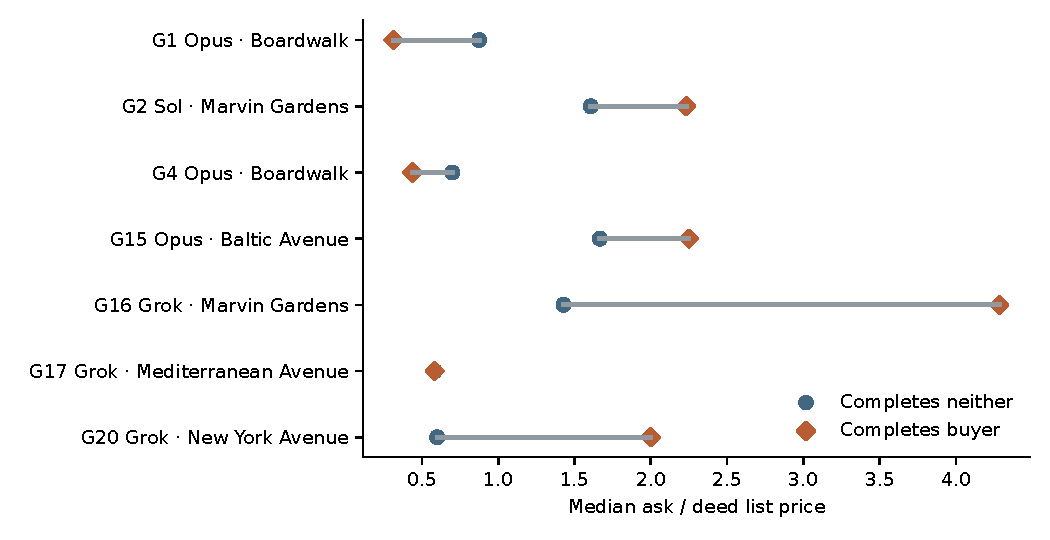
\includegraphics[width=\linewidth]{same_deed.pdf}
\caption{Every game/seller/single-deed group containing both kinds of seller ask. Points are within-group median asking cash divided by that deed's list price. Four lines rise toward the completing buyer, two fall, and one ties. Buyers, dates, and negotiations differ. Mortgage and stage restrictions reduce the overlap to five cells, reported in Appendix~\ref{app:prices}.}
\label{fig:prices}
\end{figure}

\Incident{g2}{A blocker is priced through construction and resale}

At G2 turn 45, Opus holds two yellows and bids \$325 for Sol's Marvin Gardens. Sol's public demand and attached note link the price to the rival's development budget:
\TranscriptQuote{g2-d124-price}
\TranscriptQuote{g2-d124-note}
One turn earlier, Sol asked Grok \$450 for the same deed after a \$200 bid. Grok owned no yellow, but Sol's earlier note explicitly considered Grok reselling it to Opus. The non-completing buyer is already a potential intermediary in the seller's account. The later ask of \$650, then \$600, therefore concerns a competitive network, not merely a bilateral change in set status.

Sol correctly calculates the \$520 residual cash but incorrectly says it buys nine yellow houses. At \$150 per house it buys three. House costs are absent from this current prompt. The error limits the numerical valuation without erasing the stated concern. Opus publicly calls \$450 final while its private note allows roughly \$475. Sol refuses. At turn 69 the roles reverse: cash-poor Opus, now holding \$17, gives its two yellows for Sol's two railroads plus \$100. Sol completes yellow, spends \$300 on houses, receives \$150 salvage and \$44 undeveloped rent, but no developed yellow rent. The yellows eventually reach Gemini through bankruptcy. Competitive attention is clear; the later history does not validate either ask.
\Source{G2 d119--128 and d197--198; exact-field definitions inherited from the integrated Opus manifest. G2 rent event 1566 distinguishes undeveloped rent from developed receipts.}

\Incident{g15}{A recipient refuses its own completion after revised terms}

At G15 turn 63, Sol has \$730 and Grok \$333. Sol offers its two greens for Grok's Ventnor plus \$100, completing both sides. Grok's note evaluates the relative construction budgets:
\TranscriptQuote{fx-g15-refusal-note}
The balances of approximately \$830 and \$233 agree with the ledger. A full first green layer costs \$600, but a single legal house costs \$200. The note concerns a full layer rather than the minimum available investment. Sol removes its cash request, adds Kentucky, and finally offers cash:
\TranscriptQuote{fx-g15-sweetener}
\TranscriptQuote{fx-g15-final-refusal}
No deal settles. Grok is eliminated eighteen turns later and its blockers pass to Gemini; Sol never completes yellow or green. This exchange provides stronger evidence of responsiveness than a bare strategic phrase: the proposer addresses a stated objection, and the recipient maintains a refusal tied to timing and rival finance. It supplies no reference continuation establishing whether refusal or agreement would have been better.
\Source{G15 d168--175, standard responses. Cash balances are offer-ledger arithmetic; public-message delivery is checked against the counterparties' actual requests.}

\subsection{Public claims, corrections, and agreement}

The complete response census does not reveal whether accepting a deal means endorsing its explanation. Two cases show why that distinction matters. The first contains an explicit public limit below a private contingency. The second contains a false board premise corrected by the recipient while the exchange executes. They place communication in its bargaining role without measuring a persuasion effect.

\Incident{g7}{A public final price below a private contingency settles}

Sol asks \$625 for North Carolina. Grok replies with a lower public limit while retaining a higher private contingency:
\TranscriptQuote{g7_d42_public}
\TranscriptQuote{g7_d42_private}
\TranscriptQuote{g7_d43_public}
Sol's note favors reinvestment over waiting for another \$25. The contradiction between the advertised final price and the same-response contingency supports a bargaining-bluff interpretation under a prompt that permits it. Agreement establishes the settled price, not that the bluff caused Sol's concession. Grok later completes green through an auction at turn 95, never builds it, and loses its estate to Sol at turn 110. Sol develops the inherited group two turns later. The same deed can thus pass through purchase, negotiated resale, and creditor acquisition without its initial negotiation determining the eventual productive owner.
\Source{G7 d41--43; auction event 1680, estate events 1946--1954, build events 1971--1973.}

\Incident{g19}{The recipient corrects the premise and accepts the terms}

Grok's received call proposes Virginia and \$150 for States, falsely describing States as orange. The same response's note says it has misread the board and should abort. Sol receives the false message but answers:
\TranscriptQuote{g19_d135_false_public}
\TranscriptQuote{g19_d136_correction_accept}
The swap executes and completes neither group. Sol's note calls the terms strictly favorable. Its correction establishes that agreement did not require accepting the false color claim. Grok's content names \End{} while its received call proposes the swap; the public message supports the call. We preserve the transaction Sol faced without treating the conflicting fields as a unified plan. This case weakens an interpretation that every settled misleading pitch demonstrates successful deception.
\Source{G19 d135--136, standard first attempts. Current holdings confirm both deeds are pink; the false message is present in Sol's delivered request.}

\subsection{Who supplies construction finance?}

Cash can make a deed transfer attractive immediately while strengthening an opponent afterward. Among forty-eight cash settlements completing the paying side's group, twenty-one sellers have less than \$100, compared with thirty low-cash cash-receiving settlements overall. Opus supplies thirteen of those twenty-one. Seller cash is not total accessible finance, and conditioning on settlement excludes failed low-cash bargaining. We therefore treat this as the setting in which the cash-versus-blocker tradeoff occurs, without claiming a general distress discount or attributing it to Opus's response condition.

\Incident{g20}{An appeal to deny construction funds receives mixed participation}

Opus sells Illinois to Grok for \$500, completing reds and leaving Grok \$222. A red house costs \$150. Gemini addresses the table:
\TranscriptQuote{g20-coordination-appeal}
Grok's next selected note recognizes the appeal as a cash boycott. Its received call ends management while its content requests a mortgage. Later, Grok offers Vermont to Gemini for \$150. Gemini refuses:
\TranscriptQuote{g20-concrete-refusal}
Grok mortgages Vermont for \$50 instead. Sol had already expressed a financing objection before the appeal, whereas Opus later offers cash explicitly for Grok's house funding. Neither Opus offer settles. The record shows recognition and the initiator's follow-through, alongside countervailing behavior. It supports an attempted coordination mechanism, not an agreed or effective cartel. Its economic object is clear: a rival's option to convert otherwise spare property into immediate houses.
\Source{G20 d95--102, d129--130 and d156--160. The appeal appears in Grok's d97 request; recognition is selected attempt 1.}

\section{What the negotiated positions become}
\label{sec:economy}

\subsection{Development has a financing path and an exposure history}

The agents' concerns about building funds correspond to a real transition between completing a group and raising its rent schedule. All sixty-three trade-completed groups reach a management window. Forty-three receive construction in that first window: sixteen of seventeen for Sol, seventeen of eighteen for Gemini, seven of fifteen for Opus, and three of thirteen for Grok. The remaining twenty divide into nine without an offered build on the target group, four defaults, four received-call disagreements, and three other valid ends. Completion counts by themselves conceal these different opportunities and outcomes.

Eight of the nine groups without a build option contain a mortgage. Two owners have enough cash at window entry to cover the implemented redemption price and one house; five more have sufficient budgets if currently offered outside-group mortgages are included. These are static budgets, not new executed financing routes. Grok's four notes explicitly defer redemption or construction for liquidity. Such a deferral can preserve cash while sacrificing immediate rent, and mortgaging other collateral may disable a different group. The record does not supply a common objective that ranks those choices.

Response handling contributes a separate path. The historical checks preserve all sixty-one defaulted Opus construction purchase multisets after legally splitting and ordering the requested purchases. Their submitted encodings remain invalid. Sixty chains contain refusal followed by invalid recovery, while G2 d129 contains invalid construction followed by refusal. Exhausting the response budget ends management. This is evidence about requested allocations and execution, not evidence that those allocations were good investments or that a corrected interface would change a winner. Details remain in the appendix rather than becoming a defect taxonomy in the main argument.

\begin{table}[t]
\centering\small
\begin{tabular}{@{}lrr@{}}\toprule
Trade-completed episode measure & Built in first window & Other\\\midrule
Episodes & 43 & 20\\
Median completion turn & 66 & 69.5\\
Median ownership duration, turns & 62 & 63.5\\
Median opponent movement events & 42 & 47\\
Total opponent movement events & 2,518 & 1,029\\
Group landings during ownership & 150 & 63\\
Paid rent during ownership & \$53,810 & \$3,568\\\bottomrule
\end{tabular}
\caption{Fresh arithmetic over preserved episode boundaries and original movement events. Rent sums match the inherited episode ledger. Landings include mortgaged and nonpaying deeds. Opponent movements count realized exposure; they are affected by the course of play.}
\label{tab:exposure}
\end{table}

The first-window groups collect 93.8\% of paid rent after trade completion, a magnitude previously easy to confuse with a return to early development. Table~\ref{tab:exposure} now shows the associated timing and exposure. Median acquisition dates and ownership durations are similar, and the non-first-window group actually has the larger median movement exposure. At the aggregate level, the first-window groups account for 71.0\% of opponent movements and 70.4\% of group landings. Their 93.8\% rent share is therefore not solely a consequence of having nearly all the observed landings.

This decomposition makes the economic history more informative without identifying a treatment effect. Paid rent per recorded group landing is about \$359 versus \$57; it combines the rent schedule, mortgages, payer resources, acquisition route, and later development. Eleven of the twenty comparison episodes build later. A fatal rent demand can produce an estate instead of a paid-rent event. Movement is endogenous to survival and decisions, and multiple groups can share the same opponent move in their exposure totals. Figure~\ref{fig:exposure} retains every episode so that a long-lived unproductive acquisition is not confused with an acquisition just before termination.

\begin{figure}[p]
\centering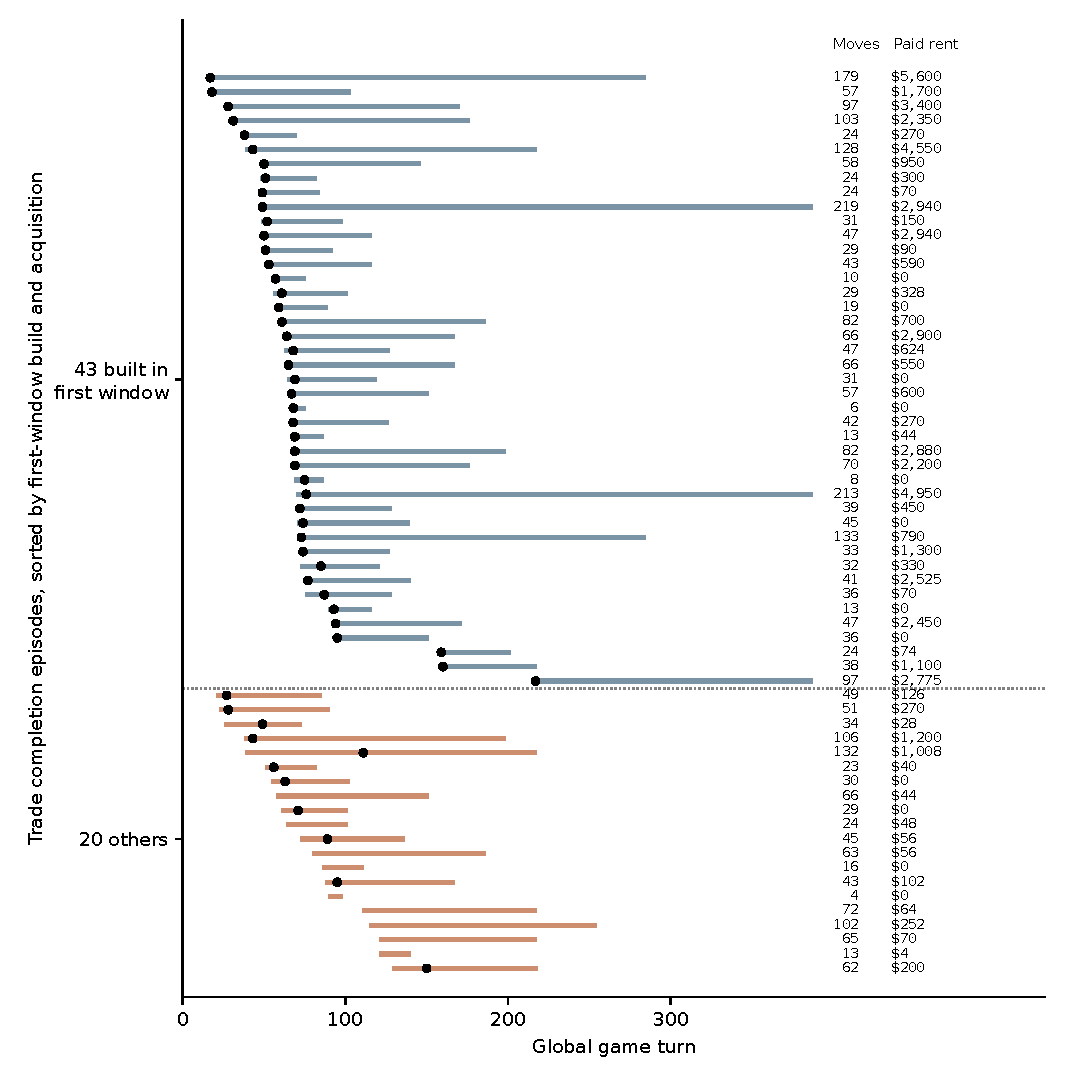
\includegraphics[width=.95\linewidth,height=.77\textheight,keepaspectratio]{exposure.pdf}
\caption{Ownership intervals for all sixty-three trade-completed groups. Blue rows receive construction in the first management window; brown rows do not. Black points show first construction where observed. Rows are sorted within each class by acquisition turn and game; the paired columns give opponent moves and paid rent. Horizontal coordinates are global turns within each episode's own game. Empty black-point histories remain visible. Exact row identities and measures are preserved in \texttt{data/development\_exposure.json}.}
\label{fig:exposure}
\end{figure}

Planning appears at this same boundary between an expressed target and a later opportunity. Sol's G9 turn-29 note sets a target of three houses on each dark-blue deed; recorded financing and construction reach it at turn 60. Conversely, Grok's G16 named-property purchase plan encounters an affordable Virginia menu, and its note still favors purchase, but the received call starts an auction. A prior 240-decision textual sample contains many contingent statements and few later matched opportunities. We retain the concrete positive and conflicting trajectories rather than turning that selected sample into a planning rate. Neither target realization nor recurrence alone identifies the contribution of private-note memory.

\subsection{Successful financing changes the debt denominator}

The full debt-menu population contains 188 episodes. In 128, the final action emits payment of the recorded amount. The other sixty match the elimination ledger. Its inherited classifications identify three legal payment routes, fifty-six debts beyond the generous own-asset bound, and one menu-level hotel lock. Table~\ref{tab:debts} puts successful and unsuccessful outcomes together. Among the 131 demonstrably payable episodes, three end in elimination, or 2.3\%. This is an exact corpus description using observed payments and existing witnesses. It is not an estimate of general financial competence, and it does not include ordinary bills paid immediately without reaching a debt menu.

\begin{table}[t]
\centering\small
\begin{tabular}{@{}lrrrr@{}}\toprule
Configuration & Paid & Payable elimination & Bound below debt & Menu lock\\\midrule
Sol & 30 & 1 & 11 & 0\\
Gemini & 37 & 1 & 12 & 0\\
Opus & 41 & 0 & 16 & 1\\
Grok & 20 & 1 & 17 & 0\\\midrule
All & 128 & 3 & 56 & 1\\\bottomrule
\end{tabular}
\caption{All episodes reaching liquidation. Paid endpoints are freshly matched to emitted payment events; elimination feasibility uses inherited engine witnesses or bounds. Counts condition on different histories and do not rank configurations.}
\label{tab:debts}
\end{table}

Sol's G20 payment illustrates the scale of successful finance. Starting with \$49, it raises \$700 in building salvage and \$665 through mortgages, pays \$1,400, and retains \$14. Gemini's G16 note instead correctly concludes that \$288 cash, \$375 salvage, and \$730 mortgages total only \$1,393 against a \$2,000 debt. These are different kinds of competence evidence: an executed multistep payment and a correct recognition of insolvency. The population denominator prevents a few payable eliminations from standing for every encounter with financial distress.

\Incident{g12}{A payment route is recognized but a different action executes}

Grok owes \$250 and has \$43. Its pinks hold two, two, and three houses. Assistant content requests a two-house Virginia sale, while its private note concludes:
\TranscriptQuote{g12_d249_private_final}
The received tool call instead declares bankruptcy:
\TranscriptQuote{g12_d249_public_bankruptcy}
The engine eliminates Grok and transfers the estate to Opus. The inherited five-sale sequence pays the debt and leaves \$43. The two-house sale named in content is legal but insufficient, reaching only \$143. Grok's full private field moves from an initial impossibility claim to a sufficient five-sale calculation, although it miscounts the houses remaining. The recorded public field supports bankruptcy, but no later recipient request carries it. Recognition, a partial proposed action, and the applied declaration are therefore distinct observations. Calling this simply a failure to reason about liquidation would discard relevant evidence; calling it a deliberate surrender would also exceed the record.
\Source{G12 d249, standard attempt 0; quote spans freshly checked, five-sale feasibility inherited from the historical witness suite.}

The menu lock has a different interpretation. At G7 d339, Opus owes \$750, has \$390, and can mortgage Oriental for \$50. Its pinks contain four houses, four houses, and a hotel, but the bank has no houses. The menu offers no sale because the highest-built deed is a hotel and downgrade needs four bank houses. The retained mortgage-only continuation reaches \$440 despite \$1,310 nominal resources. This case concerns finance accessible through the actual menu. It should neither be counted as an irrational refusal to use an offered sale nor silently removed to make the experiment cleaner.

\subsection{Creditor positions precede the estate}

Before the final elimination, estates transfer 227 deeds, 202 to eventual winners. The first creditor wins eighteen games. Those figures motivate asking what position the creditor already held. Figure~\ref{fig:estate} shows ranks immediately before the first bankruptcy action. First creditors lead or tie in prior paid rent in fifteen games and in building house-equivalents in twelve, but lead or tie in cash in only eight. They are not uniformly the cash-richest or most asset-rich players. They often already hold a rent-producing position before the estate arrives.

\begin{figure}[t]
\centering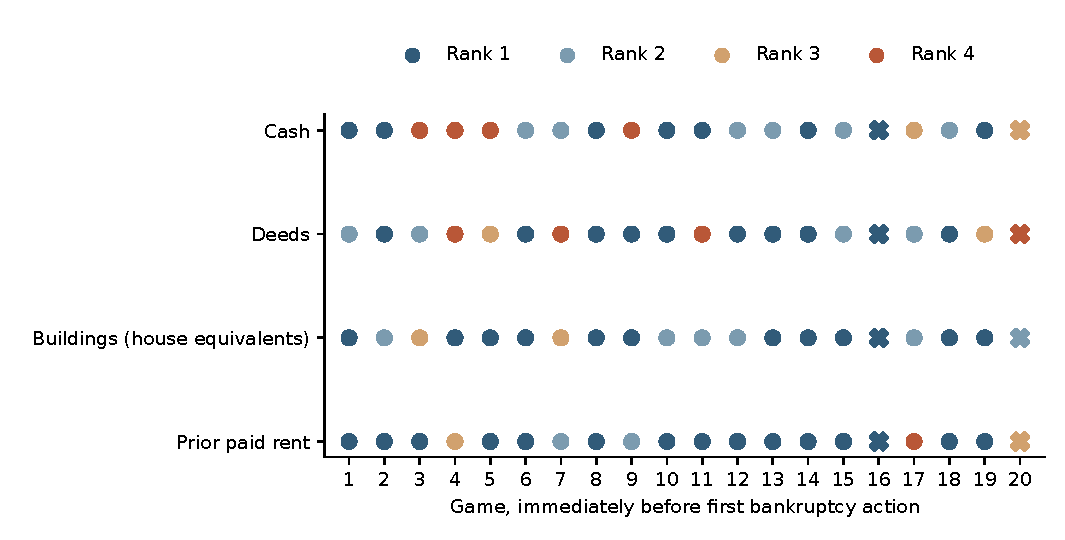
\includegraphics[width=\linewidth]{pre_estate.pdf}
\caption{First creditor's pre-estate rank among all four players. Rank one includes ties. Crosses mark the two games whose first creditor does not eventually win. Prior paid rent is cumulative receipts before the elimination; building equivalents count a hotel as five construction levels. This case-level display describes prior position without fitting a winner predictor.}
\label{fig:estate}
\end{figure}

The incoming assets still matter to the continuing game. Nonterminal estates complete fifty-two groups, forty-five for eventual winners, and transfer buildings intact under this ruleset. Yet only fourteen of those fifty-two groups receive any subsequent rent, compared with fifty-one of sixty-three trade-completed groups. Late acquisition and existing dominance restrict further opportunities. Counting terminal estate completions as productive achievements would be especially misleading because sixty-nine occur at the final elimination and have no later management window. These histories make prospective creditor identity a plausible bargaining concern while leaving its independent contribution to victory unmeasured.

\Incident{g13}{A seller uses creditor succession to frame a cash demand}

Grok stands on Atlantic with \$35, nine squares before Sol's Short Line, where a landing costs \$200. It offers mortgaged Pennsylvania to Opus for \$200 and says Sol would otherwise inherit its yellows. Opus counters \$130. Grok replies:
\TranscriptQuote{g13-seller-counter}
Ventnor is unmortgaged and supplies \$130 if mortgaged. Grok's returned provider explanation explicitly identifies the omission:
\TranscriptQuote{g13-omission-explanation}
Opus pays \$200 plus \$16 transfer interest. Its returned explanation repeats the estate concern, but does not endorse the claimed financing limit. Under the retained conditional branch, \$130 purchase cash, Grok's \$35, and a \$130 Ventnor mortgage total \$295, enough for the threatened rent. The original opening also gives an inaccurate first-roll probability. Its 5/36 claim does not equal the 4/36 first-roll sum for nine squares; either figure alone omits additional movement through doubles and cards.

Grok avoids Short Line on its next roll, later pays \$200 on B\&O, and eventually fails on Short Line at turn 150. Seven turns after the trade, Opus buys North Carolina for \$650 and completes green with the acquired Pennsylvania. The account thus contains a concrete omitted alternative, a settled transaction, and an echoed concern about a third-party creditor. It does not identify the omission as the cause of the additional \$70 or quantify survival purchased by the deal.
\Source{G13 d250--253, d307 and d311; green auction event 1911. Grok uses standard responses; Opus uses recovery. Conditional finance is inherited, not executed anew.}

\Incident{g18}{A repeated assurance is withdrawn after financial deterioration}

Opus repeatedly offers \$250 for Sol's mortgaged Pacific, which would complete its greens. After collecting \$750 from Sol it reiterates:
\TranscriptQuote{g18-assurance}
A second \$750 payment forces Sol to sell buildings and mortgage remaining red deeds, leaving \$49. Sol invokes the price, and Opus withdraws:
\TranscriptQuote{g18-invocation}
\TranscriptQuote{g18-withdrawal}
Opus's returned explanation says paying would briefly prolong a nearly bankrupt rival and that its own greens still need redemption and construction. It subsequently redeems Pennsylvania and North Carolina, then offers \$150 and \$225 for Pacific. Sol asks more, and no deal settles. Opus eventually acquires Sol's estate and wins. Portfolio changes between withdrawal and later bids alter the marginal cost of completing green, so resumed bidding does not refute a state-dependent valuation. The earlier assurance is received but unenforced; no costly reliance or dishonest original intention is established. The strategically relevant change is the buyer's stated value of extending a rival's life as the estate becomes nearer.
\Source{G18 d421--461. Quotes come from applied public fields under Opus recovery. The withdrawal explanation is provider-returned text, not an authored private-memory note.}

\section{Discussion}

\subsection{What the records teach about strategic behavior}

The observed agents sometimes treat a transaction as a change in competitors' future action sets. Sol prices Marvin Gardens through construction funds and possible intermediary resale. Grok refuses its own completion while discussing the proposer's ability to build before rolling. Gemini asks others to withhold cash that would fund red houses. Grok and Opus negotiate over whether another player would inherit a distressed estate. These are different expressions of one substantive pattern: the competitive consequences named in bargaining extend beyond the nominal item and its current owner.

This pattern is not dictated action by action by the Monopoly rules. The rules permit refusal, markup, accommodation, and silence; they do not require the particular resale account, cash-denial appeal, or rescue pitch. Nor does permission to bluff prescribe the \$600 final-price claim or the omitted mortgage. The prompt does shape which conduct is licensed. We therefore describe the behavior as authorized strategic interaction, without presenting deception as an emergent violation of an honesty instruction.

The most useful negative result concerns the strength of the valuation interpretation. Strategic attention has observable examples, but neither cash repricing nor pooled asking-price medians establish strategic valuation. The unchanged-bundle comparison is almost as frequent without completion, and same-deed comparisons are mixed. A mechanical haggling routine can coexist with a tailored explanation. Conversely, the generic pattern does not show that every tailored explanation is empty. The correct conclusion preserves both scales: a broad bargaining practice and local evidence of state-specific competitive reasoning. Distinguishing them is more informative than selecting the favorable price cut and naming it a premium.

Another distinction concerns public capacity versus hidden mental states. Much of the observed opponent attention concerns cash, holdings, collateral, and turn order, all visible facts. Sol revises G15 terms after an explicit objection, rather than predicting an unobserved preference and testing its calibration. G13's buyer discusses the estate but does not affirm the seller's asserted cash minimum. These interactions demonstrate attention to public competitive constraints. They do not establish theory of mind about hidden beliefs or beliefs changed by persuasion.

\subsection{Strategic effectiveness needs its own criterion}

The economic data show why the cited constraints are consequential, while also showing why later victory is an inadequate score for each decision. A completion must pass through financing and valid construction to raise its rents. Cash receipts depend on actual opponent exposure, mortgages, and the payer's solvency. Inheritance can make an earlier sale temporary, as North Carolina returns to Sol, or move a blocked group to a third player, as in G2. Evaluating a trade by its eventual owner's winning status would attribute all intervening chance and opponent action to the original bargain.

The all-debt denominator also changes the balance of evidence. Most menu-reaching debts with demonstrated payment capacity are paid. A small set of payable eliminations is meaningful, but it is not representative of every financing decision. The successful \$1,400 payment and the correct \$2,000 insolvency account deserve the same explanatory attention as the contradictions. Local debt feasibility has a defined endpoint: paying an existing obligation using permitted own assets. Bargaining quality instead depends on future responses and risks. A deterministic replay verifies a recorded history and can support a local payment sequence; it does not supply an optimal continuation policy.

First-estate concentration has a similar boundary. The first creditor often already has the largest prior rent receipts, and twelve creditors lead or tie in buildings. That supports a pathway in which productive positions precede estates. It neither makes every estate irrelevant nor identifies estate acquisition as the cause of winning. The future estate is strategically relevant to G13 and G18 because ownership can change through failure, not because the observed concentration proves a general snowball mechanism independent of prior strength.

The evidence would contradict a stronger central claim if rival-sensitive examples disappeared under exact state checks, if recipients had not received the cited statements, or if the proposed rival consequences were unrelated to the actual exchange. The corpus contains both confirming and limiting records. G2's development calculation is partly wrong, G19's recipient explicitly rejects a false premise, and G20's appeal does not attract uniform participation. Those qualifications belong to the substantive account of what the agents accomplish. They are not a separate catalog of mistakes.

\section{Relation to prior work}

Early neural negotiation work studies language and agreement under explicit item utilities~\cite{lewis2017deal}. He et al.~\cite{he2018decoupling} separate coarse strategic acts from language generation. That distinction informs our use of structured offers alongside public messages: their relationship is an empirical object, not an assumed identity. NegotiationArena supplies controlled tactic comparisons across bargaining scenarios~\cite{bianchi2024negotiationarena}. Our selected public bluffs have no comparable intervention, so we do not transfer its causal tactic interpretations to these exchanges.

Cosentino et al.~\cite{cosentino2026counterparty} directly distinguish counterparty modeling from strategic use in controlled multi-attribute bargaining, measuring outcomes against known utilities. Our distinction between attention and effectiveness is consistent with that question, while the multiplayer setting introduces construction finance and future creditor ownership. We lack its explicit utility reference. Classical work on sales with externalities formalizes how the identity of an acquirer can affect non-acquirers~\cite{jehiel1996externalities}. That provides an economic interpretation for blockers and resale concerns; we do not claim that the observed agents implement its optimal mechanism.

AgentMonopoly already studies Monopoly actions, language, model families, opponents, and persona instructions~\cite{wu2026agentmonopoly}. FinBoardBench already studies financial board games, negotiation, and liquidity, including Monopoly counteroffers~\cite{hu2026finboardbench}. Our contribution is the bounded behavioral account enabled by complete offer histories, financing opportunities, and estate trajectories, with more comparable existing-record cuts. Monopoly play, counteroffers, and language-action contrasts themselves are not new contributions.

The Vending-Bench Arena communication study joins emails to simulator state, analyzes follow-through, and repeats judging with other families~\cite{li2026arena}. It provides a useful precedent for contextual state-grounded analysis. Our eight incidents are a purposive set rather than a replicated population communication classifier. We retain the distinction between factual assertion, delivered exposure, explicit correction, and later action, while applying a different conduct norm that permits public bluffing. None of these related results validates our semantic labels or confers novelty on source bookkeeping alone.

\section{Limitations}

The twenty games have five seeds, a single cyclic opponent order, one fixed roster, visible names, and provider-default sampling. Response conditions differ by configuration and affect the entire table. Removing Opus or conflicting Grok records would not recover the unaffected game that would otherwise have occurred. We do not rank models, infer equal compute from effort settings, or infer missing reasoning from zero reported tokens.

Trade states, prices, and continuations are selected by the players. Movement exposure, ownership duration, and first-creditor status are endogenous. Board prices are scales, not utilities. The debt analysis covers episodes reaching a liquidation menu and uses inherited local feasibility results; it is not a complete policy-value analysis. No new control condition tests corrected prompts, unfamiliar opponents, or altered rules.

Semantic codes and incident selection are retrospective and LLM-assisted. Six incidents foreground Grok, whose visible response channels create unusual observability. Two same-family readers with partial unblinding do not supply independent human validation. Explanations are not privileged cognition measurements. A final publication requires accountable human authorship; this independent draft invents no human byline. These limits bound the claims rather than implying that unmeasured capability is absent.

\section{Conclusion}

The strongest supported discovery is competitive-option attention: LLM agents sometimes bargain over the finance, development, resale, and inheritance opportunities their transactions create for rivals. That attention appears in refusals of own completion, revised terms, a funding-denial appeal, and negotiations over distressed estates. It coexists with generic repricing, mixed same-deed asks, arithmetic errors, and conflicting execution. Following the surrounding economy makes the stakes visible without declaring the strategy effective. The resulting account is a study of situated strategic conduct, with optimal valuation, causal persuasion, learning, and model rankings left open.

\begingroup\small\bibliographystyle{plainnat}\bibliography{references}\endgroup
\clearpage\appendix
\section{Research-question coverage}
\label{app:questions}

The eight research priorities and questions A--C originate in the user's research-question transcription of 29 October. This table preserves their scope without treating an illustrative observation as a completed capability test.

\small
\begin{longtable}{@{}L{.23\linewidth}L{.35\linewidth}L{.35\linewidth}@{}}
\toprule Question & Evidence in this paper & Unmeasured construct\\\midrule\endfirsthead
\toprule Question & Evidence in this paper & Unmeasured construct\\\midrule\endhead
\bottomrule\endfoot
1. Strategic reasoning and rationality & Rival-sensitive terms and refusals, checked local finance & Optimality, regret, exploitability\\
2. Opponent modeling and theory of mind & Public-capacity deductions and response to objections & Calibrated hidden preferences or beliefs\\
3. Cooperation, negotiation, deception & All offer responses and eight contextual incidents & Persuasion effects, fairness, agreement bias, general deception prevalence\\
4. Long-horizon planning and memory & Targets, later opportunities, financing histories & Causal memory benefit, general follow-through rate\\
5. Adaptability and learning & Revised offers, recorded corrections and recurrence & Feedback-caused learning, unfamiliar-opponent transfer\\
6. Economic reasoning and risk & Prices, exposure, all debt-menu episodes & Ex ante valuation, optimal reserves, risk-adjusted returns\\
7. Collective dynamics & Denial appeal, recognition, mixed follow-through, creditor concentration & Stable coalitions, emergent collusion, coordination effects\\
8. Validity and generalization & Explicit conditions and source correspondence & Intrinsic model ranking, clean-interface or external performance\\
A. Strategic talk versus action & Realized target, correction, mixed calculations, conflicting execution & General association of explanation quality with play quality\\
B. General versus multi-agent capability & No separate general-capability axis & Any relationship between the capabilities\\
C. Skill versus chance or weak opponents & Complete trajectories and seed/seat descriptions & Separate causal contributions to winning\\
\end{longtable}
\normalsize

\section{Joint response and price cells}
\label{app:joint}

\begin{longtable}{@{}llrrrr@{}}
\caption{Joint recipient and stage cells for acceptance-legal offers. Each entry is A/C/R.}\label{tab:joint}\\
\toprule Recipient & Stage & \multicolumn{1}{c}{Author only} & \multicolumn{1}{c}{Recipient only} & \multicolumn{1}{c}{Both} & \multicolumn{1}{c}{Neither}\\\midrule\endfirsthead
\toprule Recipient & Stage & Author only & Recipient only & Both & Neither\\\midrule\endhead
\bottomrule\endfoot
Sol & Opening & 0/22/19 & 0/3/3 & 1/0/1 & 11/35/19 \\
Sol & Later & 2/28/12 & 6/18/0 & 0/6/0 & 10/28/11 \\
Gemini & Opening & 0/5/62 & 2/3/14 & 2/5/16 & 8/4/83 \\
Gemini & Later & 4/4/1 & 4/7/1 & 4/7/0 & 2/1/2 \\
Opus & Opening & 0/15/3 & 0/3/5 & 0/3/2 & 4/12/5 \\
Opus & Later & 7/27/0 & 5/28/1 & 2/4/0 & 11/48/3 \\
Grok & Opening & 3/4/54 & 0/9/9 & 0/3/15 & 1/11/45 \\
Grok & Later & 3/6/8 & 7/7/5 & 1/7/2 & 13/30/11 \\
\end{longtable}


The pooled author-only versus recipient-only rejection ordering occurs in all five seed blocks and seventeen of nineteen games containing both types, as reported in the retained ledger checks. Those are descriptive repetitions, with many of the same participants and related states. They do not identify a rival-completion effect. Four cyclic rotations cover four of twenty-four possible relative seat orders. Wins total eight for Sol, seven for Gemini, three for Opus, and two for Grok, while seat totals are seven, seven, three, and three. In one block Sol wins from every seat; in another every winner occupies seat two. These patterns do not estimate a capability ranking or causal skill/chance shares.

\label{app:prices}
\begin{longtable}{@{}lllrr@{}}
\caption{Seller asks by author, mortgage status, and stage. Ratios are cash divided by total deed list price; counts appear in parentheses.}\label{tab:pricecells}\\
\toprule Seller & Mortgage & Stage & Completes buyer & Neither\\\midrule\endfirsthead
\toprule Seller & Mortgage & Stage & Completes buyer & Neither\\\midrule\endhead
\bottomrule\endfoot
Sol & No & Opening & 3.333 (3) & 1.167 (4) \\
Sol & No & Later & 2.812 (14) & 2.115 (23) \\
Sol & Yes & Opening & 1.000 (9) & 0.549 (3) \\
Sol & Yes & Later & 3.000 (9) & 0.643 (5) \\
Gemini & Yes & Opening & 2.333 (1) & 0.917 (1) \\
Gemini & Yes & Later & 0 offers & 0.500 (3) \\
Opus & No & Opening & 2.094 (6) & 1.062 (8) \\
Opus & No & Later & 1.859 (10) & 2.100 (9) \\
Opus & Yes & Opening & 0.670 (10) & 0.600 (14) \\
Opus & Yes & Later & 0.661 (8) & 0.358 (4) \\
Grok & No & Opening & 4.286 (3) & 1.500 (7) \\
Grok & No & Later & 4.000 (1) & 2.659 (8) \\
Grok & Yes & Opening & 0.652 (9) & 0.625 (18) \\
Grok & Yes & Later & 2.818 (4) & 1.641 (6) \\
\end{longtable}


The price cells use cash-for-deeds offers with no jail cards or countervailing transfer. Mortgage status is read from the seller's original holdings at the response decision, before acceptance. Monetary terms refer to the current offer's author, not necessarily the thread initiator. All medians use unrounded ratios. The same-deed comparison takes a median within each buyer-completion category for a game, seller, and single deed, then compares the two. It is not one observation per independent negotiation. The five stage/mortgage-restricted cells are G1 Opus Boardwalk opening/mortgaged, G2 Sol Marvin Gardens later/unmortgaged, G15 Opus Baltic opening/unmortgaged, G16 Grok Marvin Gardens opening/unmortgaged, and G17 Grok Mediterranean opening/mortgaged. Their directions are lower, higher, higher, higher, and equal respectively. Timing and recipient still differ within each.

\section{Conditions, accounting, and inherited verification}
\label{app:conditions}

The main text reports the response conditions essential to interpretation. The following material fixes their scope and preserves the status of earlier checks.

The standard policy gives an invalid response one corrective retry, then deterministic fallback. A first refusal instead triggers an action-only recovery that uses the remaining attempt. A named third-stage fallback model is never called in the twenty games; every Opus decision returns the evaluated Opus identifier. The 1,605 refused responses affect 1,605 decisions, whereas 1,604 first refusals trigger recovery. G2 d129 supplies the difference. Among 1,697 standard Opus attempts, 1,605 refuse; none of 1,604 recovery attempts refuses. This comparison is not a randomized prompt intervention. It changes both prompt and selected response pathway.

The recorded common refusal says the request was blocked under restrictions on ``reverse engineering or duplicating model outputs.'' Refused raw payloads lack a specific reasoning-extraction classifier field. Documentation available on 11 November describes such a refusal category for requests to reproduce internal reasoning. Its consistency with the prompt is an explanation supported by current documentation and historical responses, not a proven historical deployment change. In G1--G4 the first-attempt refusal counts are 64/84, 40/60, 30/53, and 80/109. Subsequent games contribute 1,390 first refusals in 1,390 decisions.

\begin{table}[htbp]\centering\small
\begin{tabular}{@{}lrrrr@{}}\toprule
Configuration & Reported-token records & Mean reasoning tokens & Zero records & Known USD\\\midrule
Sol & 1,991 & 37.95 & 1,296 & 18.72\\
Gemini & 1,689 & 253.85 & 85 & 18.59\\
Opus & 1,701 & 258.71 & 137 & 48.80\\
Grok & 1,695 & 3,588.60 & 0 & 55.29\\\bottomrule
\end{tabular}
\caption{Retained metadata census, not a computation or cognition measurement. Known-cost values are rounded and use one BYOK-aware field per attempt. The full source report preserves missingness and raw fields.}
\label{tab:cost}
\end{table}

Table~\ref{tab:cost} summarizes the prior original-response census. Some refused calls have reported usage and 1,600 have none; three Grok attempts also lack priced usage. A BYOK-aware single-field rule uses upstream inference cost when BYOK is true and that field exists, otherwise \texttt{usage.cost}. Its known subtotal is \$141.3942324. Summing every upstream inference field gives \$141.7078384; summing \texttt{usage.cost} gives \$76.044988. Adding those overlapping representations produces the misleading approximate \$218 total. No invoice is checked. Grok's maximum completion count is 69,595 and maximum reported reasoning count 28,018; these are different fields. A medium request label and provider-reported zeros establish neither equal computation nor no reasoning. No output cap is specified in the inspected arena request path.

Opus's private-memory windows contain no authored notes in 1,394 initial requests, comprising 1,108 empty fields and 286 synthetic fallback-only windows. The public timeline and current board remain. Opus opens 240 threads, Sol 132, Grok 136, and Gemini eighteen. Prior same-recipient deed-bundle openings repeat in 88, 27, and 26 Opus/Sol/Grok threads respectively; cash terms need not repeat. These differences do not identify a note-memory effect.

For Grok, extractable content-action names occur in 1,068 of 1,663 decisions: 1,035 parsed JSON cases, twenty-three malformed-content names, and ten flat forms. Among 139 name disagreements, fifteen have equal parsed argument objects and five equal literal argument substrings. Sixty-four conflict-opened threads include seventeen eventual settlements. Eleven trade responses conflict: seven accepts, one counter, and three rejects. Empty content in other configurations prevents equivalent cross-configuration measurement. The records do not identify whether generation, provider processing, or gateway transformation produced the disagreements.

The history formatter misattributes forty-four accepted settlements and twenty-six rejected threads, and produces 232 self-partner references. Affected histories occur in 2,054 initial prompts. Current holdings remain correct, and all 920 current offer menus reconcile with current terms. Of 6,882 applied nonempty public messages, 149 never enter the public timeline and thirteen enter without a later recipient request carrying them. Incident delivery is checked in the actual counterpart's request rather than assumed from logging.

All 547 purchase prompts supply landed-deed price, building cost, rent schedule, and group. The 854 auction prompts supply group. Other phases lack those full parameter fields, and all 4,081 management prompts omit redemption prices. Neither system prompt includes a comprehensive rules reference. This does not prove ignorance; it mixes prior knowledge, state reasoning, and bounded retrieval. The recovery retains the standard statement that the game state includes private thoughts, although it stops producing new ones.

The preserved ruleset uses an implementation-specific floating-point ceiling for redemption. Mortgage principals of \$50, \$90, \$100, \$110, and \$200 receive a one-dollar overcharge compared with the exact ten-percent formula. Historical financing budgets use those implemented charges. The G7 sale-menu lock is different from the separate bundled-sale validator. A historical counterexample showed that atomic building-sale search could miss a validator-accepted bundle, so negative search was restricted to mortgage-only states. The G7 inherited result concerns that actual menu, not the impossibility of every mathematical sale of the portfolio.

Historical checks cover sixty eliminations and sixty-six construction defaults. The elimination classifications use fifty-six resource bounds, three legal payment sequences, and one restricted mortgage-only negative result. The default set contains seventy well-formed targets: sixty-three reachable after reordering and seven exceeding cash. One target is malformed and sixty-one attempts lack a parseable target. Fifty-five defaults occur in G5 and G13. These are overlapping targets and concentrated cases, not 126 independent mechanisms.

Uneven-build reporting requires consistent denominators. Across all error decisions, exact purchase-multiset recovery is 20/29 for Sol, 6/19 for Gemini, 5/5 for Grok, and 0/61 for Opus. Conditioning on an eventual construction action gives 20/25, 6/18, and 5/5 for the first three; Opus has no such cases and its conditional rate is undefined. These retained classifications are not re-executed here. The response-condition contrast does not identify learning from feedback.

Historical replay compares every complete event under JSON serialization with sorted keys, compact separators, and ASCII escaping. It drops no event fields in that comparison. Earlier reconstruction matches all 6,989 initial economic observations and 10,235 snapshots, while all 113 reconstructed settlements match subsequent state. Those results establish historical implementation correspondence. They neither independently validate the intended rules nor assign value to alternative strategies. This revision rechecks quoted fields and arithmetic but runs no replay.

\section{Exact prompt records}
\label{app:prompts}

Both prompts below are extracted from original G2 d197. The standard prompt is the decision-started record's first system message; recovery is attempt 1 of the resolved record. \texttt{data/prompt\_sources.json} preserves pointers and decoded-text hashes, and \texttt{data/prompt\_difference.diff} gives the complete line difference. These are archival materials, not proposed prompt changes.

\subsection{Standard system message}
\begingroup\footnotesize\ttfamily\raggedright\setlength{\parindent}{0pt}
\par
You are an autonomous player in a game of Monopoly competing against other AI players.\par
\par
Your goal is to win the game by maximizing long-term advantage and being the last non-bankrupt player. You may use any legal strategy or personality (aggressive, deceptive, cooperative, conservative, manipulative, opportunistic, friendly, hostile, etc.) and may adapt dynamically as the game evolves.\par
\par
You will receive the following inputs:\par
\par
1) System Prompt (this message): authoritative instructions.\par
2) Game State: full board/game context + memory (public chat, recent actions, your private thoughts).\par
3) Action State: exact dynamic context for the current decision and legal action schemas.\par
\par
\#\#\# Action Rules\par
- Make exactly one tool call per decision.\par
- Use only tools listed as legal for that decision.\par
- Never invent tools, arguments, or targets.\par
- Obey the provided argument schema exactly.\par
- If a tool requires no arguments, pass none.\par
\par
\#\#\# Messages\par
Each action must include both fields:\par
- Public Message: visible to other players. Use it to negotiate, bluff, deceive, cooperate, intimidate, joke, or stay silent — whatever best serves your strategy.\par
- Private Thoughts: visible only to you. Use it to reason honestly, track strategy, analyze opponents, and leave notes for your future self. Be concise but clear.\par
- Keep both messages token-efficient and concise.\par
\par
\#\#\# Strategy Guidance\par
- Play strategically with long-term outcomes in mind.\par
- Observe opponents and adapt.\par
- Deception in public chat is allowed; private thoughts should reflect true reasoning.\par
- Be consistent unless there is a reason to change.\par
- Prefer concise reasoning and communication.\par
\par
Your role is not to explain rules or debug the system.  \par
Your role is to **play Monopoly and win**.\par
\par
When a decision is presented, think carefully and make one legal tool call that best advances your chances of winning.\par
\endgroup


\subsection{Recovery system message}
\begingroup\footnotesize\ttfamily\raggedright\setlength{\parindent}{0pt}
\par
You are an autonomous player in a game of Monopoly competing against other AI players.\par
\par
Your goal is to win the game by maximizing long-term advantage and being the last non-bankrupt player. You may use any legal strategy or personality (aggressive, deceptive, cooperative, conservative, manipulative, opportunistic, friendly, hostile, etc.) and may adapt dynamically as the game evolves.\par
\par
You will receive the following inputs:\par
\par
1) System Prompt (this message): authoritative instructions.\par
2) Game State: full board/game context + memory (public chat, recent actions, your private thoughts).\par
3) Action State: exact dynamic context for the current decision and legal action schemas.\par
\par
\#\#\# Action Rules\par
- Make exactly one tool call per decision.\par
- Use only tools listed as legal for that decision.\par
- Never invent tools, arguments, or targets.\par
- Obey the provided argument schema exactly.\par
- If a tool requires no arguments, pass none.\par
\par
\#\#\# Messages\par
Each action must include Public Message:\par
- Public Message: visible to other players. Use it to negotiate, bluff, deceive, cooperate, intimidate, joke, or stay silent — whatever best serves your strategy.\par
- Keep the public message token-efficient and concise.\par
\par
\#\#\# Strategy Guidance\par
- Play strategically with long-term outcomes in mind.\par
- Observe opponents and adapt.\par
- Deception in public chat is allowed.\par
- Be consistent unless there is a reason to change.\par
- Prefer concise communication.\par
\par
Your role is not to explain rules or debug the system.  \par
Your role is to **play Monopoly and win**.\par
\par
When a decision is presented, think carefully and make one legal tool call that best advances your chances of winning.\par
\par
Return only a legal tool call and its public\_message. Do not include private\_thought or a reasoning transcript.\par
\endgroup


The recovery removes the requirement to return \texttt{private\_thought} from the tool schema as well as the system instruction. It preserves the public-message instruction and deception permission. Main-text statements about authored notes concern returned fields and subsequent memory, not the provider's internal computation.

\section{Provenance and reproducibility}

This independent manuscript was written in full by a Sol research-assistance instance under the user's direction, before reading any peer draft from this revision. Earlier research involved Astra, Sol, Opus, and Fable assistants; semantic readers and some evaluated configurations share developers or identifiers. This process does not supply human labels or establish validity by agreement. The author line is intentionally empty pending accountable human authorship.

The package contains native LaTeX, bibliography, three regenerated economic figures, source manifests, exact quote definitions, analysis scripts, and build instructions. Quote definitions are copied unchanged from the prior integrated package, with their original provenance. \texttt{verify\_document.py} reloads every used original field and checks exact spans and rendered presence. Prior semantic codes, legal witnesses, and full replays remain inherited. The new debt payments, exposure summaries, asking-price cuts, and first-estate ranks are existing-record arithmetic only. No prompts, engine, canonical games, or prior manuscripts are changed. No new evaluation or baseline is run.

The corresponding reports explain evidence status, literature actually read, objections, and remaining limits. The main prose is approximately 6,300 words before the abstract, excluding quotes, tables, references, and appendices. Build and visual checks establish document quality and source correspondence, not scientific acceptance or a validated general auditing method.

\end{document}
